% define documentclass
\documentclass[12pt, bibliography=totoc, a4paper, abstractoff, numbers=noenddot]{scrreprt}

% define used packages
\usepackage[left=4.0cm, right=2.0cm, top=3cm, bottom=3cm]{geometry}
\usepackage{bibgerm}
\usepackage{caption}
\usepackage[utf8]{inputenc}
\usepackage[T1]{fontenc}
\usepackage{graphicx}
\usepackage[ngerman]{babel}
\usepackage{lmodern}
\usepackage{listings}
\usepackage[numbers]{natbib}
\usepackage{acronym}
\bibliographystyle{alphadin}
\usepackage{float}

\usepackage{lastpage}

% advanced tables
\usepackage{array}

% header and footer
\usepackage{fancyhdr}

% links
\usepackage{url}

% internal links
\usepackage[colorlinks=true ,linkcolor=black,
			anchorcolor=black ,citecolor=black ,filecolor=black,
			menucolor=black ,urlcolor=black]{hyperref}

% mathematical formulas
\usepackage{amsmath, amssymb}

% fancy Diagrams %
\usepackage{tikz}
\usepackage{epstopdf}

% to include images side by side
\usepackage{subfigure}

% for nice bg on title page
\usepackage{eso-pic}
\newcommand\BackgroundPic{%
\put(0,0){%
\parbox[b][\paperheight]{\paperwidth}{%
\vfill
\centering

\includegraphics[width=\paperwidth,height=\paperheight,%
keepaspectratio]{images/Logo_H-BRS_background}%
\vfill
}}}

% define the programming language
\usepackage{listings}
\lstloadlanguages{Java,sh,bash,Haskell,HTML,PHP,XML}
\lstdefinelanguage{console}{
  morekeywords={},
  otherkeywords={warumgehtdasnicht>,\$}
}
\newcommand{\lstsetconsole}
{ \lstset{%language=sh,
        lineskip=-2pt,
        breaklines=true,
        language=console,
        breaklines=true,
        captionpos=b,
        commentstyle=\textit,
        keywordstyle=\bfseries,
        basicstyle=\ttfamily,
        stringstyle=\ttfamily,
        showstringspaces=false,
        frame=single,
        tabsize=2
  }
}
\lstdefinelanguage{scalaconsole}{
  morekeywords={},
  otherkeywords={scala>,\|}
}
\newcommand{\lstsetrepl}
{ \lstset{%language=sh,
        lineskip=-2pt,
        breaklines=true,
        language=scalaconsole,
        breaklines=true,
        commentstyle=\textit,
        keywordstyle=\bfseries,
        basicstyle=\ttfamily,
        stringstyle=\ttfamily,
        showstringspaces=false,
        frame=single,
        tabsize=2
  }
}
\newcommand{\lstsetjava}{
 \lstset{language=Java,
        breaklines=true,
        commentstyle=\textit,
        keywordstyle=\bfseries,
        basicstyle=\ttfamily,
        stringstyle=\ttfamily,
        showstringspaces=false,
        frame=single,
        captionpos=b,
        tabsize=2,
        literate=
        %linewidth=\textwidth,captionpos=b
        %numbers=left, stepnumber=5, numbersep=10pt
 }
}
\lstdefinelanguage{scala}{
  morekeywords={abstract,case,catch,class,def,%
    do,else,extends,false,final,finally,%
    for,forSome,if,implicit,import,lazy,match,mixin,%
    new,null,object,override,package,%
    private,protected,requires,return,sealed,%
    super,this,throw,trait,true,try,%
    type,val,var,while,with,yield},
  otherkeywords={_,:,=,=>,<-,<\%,<:,>:,\#,@},
  sensitive=true,
  morecomment=[l]{//},
  morecomment=[n]{/*}{*/},
  morestring=[b]",
  morestring=[b]',
  morestring=[b]"""
}
\newcommand{\lstsetscala}{
 \lstset{language=scala,
        breaklines=true,
        commentstyle=\textit,
        keywordstyle=\bfseries,
        basicstyle=\ttfamily,
        stringstyle=\ttfamily,
        showstringspaces=false,
        frame=single,
        tabsize=2
        %%linewidth=\textwidth,captionpos=b
        %numbers=left, stepnumber=5, numbersep=10pt
 }
}
\newcommand{\lstsethtml}{
 \lstset{language=HTML,
        breaklines=true,
        commentstyle=\textit,
        keywordstyle=\bfseries,
        basicstyle=\ttfamily,
        stringstyle=\ttfamily,
        showstringspaces=false,
        frame=single,
        tabsize=2
        %%linewidth=\textwidth,captionpos=b
        %numbers=left, stepnumber=5, numbersep=10pt
 }
}
\newcommand{\lstsetphp}{
 \lstset{language=PHP,
        breaklines=true,
        commentstyle=\textit,
        keywordstyle=\bfseries,
        basicstyle=\ttfamily,
        stringstyle=\ttfamily,
        showstringspaces=false,
        frame=single,
        tabsize=2
        %%linewidth=\textwidth,captionpos=b
        %numbers=left, stepnumber=5, numbersep=10pt
 }
}
\lstnewenvironment{code}
    {\lstset{}%
      \csname lst@SetFirstLabel\endcsname}
    {\csname lst@SaveFirstLabel\endcsname}
\newcommand{\lstsethaskell}{
    \lstset{
      language=Haskell,
      commentstyle=\textit,
      keywordstyle=\bfseries,
      basicstyle=\ttfamily,
      stringstyle=\ttfamily,
      showstringspaces=false,
      frame=single,
      flexiblecolumns=false,
      basewidth={0.5em,0.45em},
      literate={+}{{$+$}}1 {/}{{$/$}}1 {*}{{$*$}}1 {=}{{$=$}}1
               {==}{{$==$}}2 %{!=}{{$\not\equiv$}}2
               {>}{{$>$}}1 {<}{{$<$}}1 {\\}{{$\lambda$}}1
               {\\\\}{{\char`\\\char`\\}}1
               {->}{{$\rightarrow$} }2 {>=}{{$\geq$}}2 {<-}{{$\leftarrow$}}2
               {<=}{{$\leq$}}2 {=>}{{$\Rightarrow$} }2
               {\ .}{{$\circ$}}2 {\ .\ }{{$\circ$}}2 {(.)}{({$\circ$})}2
               {>>}{{>>}}2 {>>=}{{>>=}}2
               {|}{{$\mid$}}1
    }
}
\lstdefinelanguage{JavaScript}{
  keywords={typeof, new, true, false, catch,%
    function, return, null, catch, switch, var,%
    if, in, while, do, else, case, break},
  ndkeywords={class, export, boolean, throw, implements, import, this},
  sensitive=false,
  comment=[l]{//},
  morecomment=[s]{/*}{*/},
  morestring=[b]',
  morestring=[b]"
}
\newcommand{\lstsetjavascript}{
  \lstset{
		language=JavaScript,
		breaklines=true,
		commentstyle=\textit,
		basicstyle=\ttfamily,
		keywordstyle=\bfseries,
		stringstyle=\ttfamily,
		showstringspaces=false,
		frame=single,
		tabsize=2
  }
}
\newcommand{\lstsetxml}{
 \lstset{language=XML,
        breaklines=true,
        commentstyle=\sffamily,
        keywordstyle=\bfseries,
        basicstyle=\sffamily,
        showstringspaces=false,
        stringstyle=\ttfamily,
        frame=single,
        tabsize=2,
        literate=
        %linewidth=\textwidth,captionpos=b
        %numbers=left, stepnumber=5, numbersep=10pt
 }
}
\lstdefinelanguage{CSharp}{
 morekeywords = {abstract,event,new,struct,as,explicit,%
    null,switch,base,extern,object,this,bool,false,%
    operator,throw,break,finally,out,true,byte,fixed,%
    override,try,case,float,params,typeof,catch,for,%
    private,uint,char,foreach,protected,ulong,checked,%
    goto,public,unchecked,class,if,readonly,unsafe,%
    const,implicit,ref,ushort,continue,in,return,using,%
    decimal,int,sbyte,virtual,default,interface,sealed,%
    volatile,delegate,internal,short,void,do,is,sizeof,%
    while,double,lock,stackalloc,else,long,static,%
    enum,namespace,string,partial},
  morecomment = [l]{//},
  morecomment = [l]{///},
  morecomment = [s]{/*}{*/},
  morestring=[b]",
  sensitive = true
}
\newcommand{\lstsetcsharp}{
 \lstset{language=csharp,
        breaklines=true,
        commentstyle=\sffamily,
        basicstyle=\sffamily,
        keywordstyle=\bfseries,
        stringstyle=\ttfamily,
        showstringspaces=false,
        frame=single,
        tabsize=2
        %%linewidth=\textwidth,captionpos=b
        %numbers=left, stepnumber=5, numbersep=10pt
 }
}
\lstdefinelanguage{FSharp}{
  morekeywords={abstract,and,as,assert,base,begin,%
    class,default,delegate,do,done,downcast,downto,%
    elif,else,end,exception,extern,false,finally,for,fun,%
    function,if,in,inherit,inline,interface,internal,lazy,%
    let,match,member,module,mutable,namespace,%
    new,not,null,of,open,or,override,private,public,rec,%
    return,static,struct,then,to,true,try,type,upcast,use,%
    val,void,when,while,with,yield,asr,land,lor,lsl,lsr,lxor,%
    mod,sig,atomic,break,checked,component,const,%
    constraint,constructor,continue,eager,event,external,%
    fixed,functor,global,include,method,mixin,object,%
    parallel,process,protected,pure,sealed,tailcall,trait,virtual,volatile},     
  sensitive=false,
  morecomment=[l][\color{greencomments}]{///},
  morecomment=[l][\color{greencomments}]{//},
  morecomment=[s][\color{greencomments}]{{(*}{*)}},
  morestring=[b]"
}
\newcommand{\lstsetfsharp}{
 \lstset{language=fsharp,
        breaklines=true,
        commentstyle=\sffamily,
        basicstyle=\sffamily,
        keywordstyle=\bfseries,
        stringstyle=\ttfamily,
        showstringspaces=false,
        frame=single,
        tabsize=2
        %%linewidth=\textwidth,captionpos=b
        %numbers=left, stepnumber=5, numbersep=10pt
 }
}

%set default pagestyle
\pagestyle{empty}

\setlength{\parindent}{0pt}
\setlength{\parskip}{12pt}

% #####
% #
% # START config area
% #
% #####

\newcommand{\HEADER}[0]{H-BRS, WS 2020 / 2021}
\newcommand{\PAGENUMBERS}[0]{\pagemark}
\newcommand{\DATE}[0]{\today}

\newcommand{\AUTHOR}[0]{Tom Gehder}
\newcommand{\MATNR}[0]{9035924}
\newcommand{\STREET}[0]{Weberstraße 79}
\newcommand{\ZIP}[0]{53113}
\newcommand{\TOWN}[0]{Bonn}

\newcommand{\REFERENT}[0]{Prof. Dr. Harm Knolle}
\newcommand{\KOREFERENT}[0]{Prof. Dr. Max Mustermann}

\newcommand{\TITLE}[0]{Programmierschnittstellen und ArangoDB (MM)}
\newcommand{\COURSE}[0]{Studiengang: Informatik}
\newcommand{\TYPE}[0]{Projektarbeit}
\newcommand{\COMPLETION}[0]{Master of Science}


% #####
% #
% # END config area
% #
% #####

% Hurenkinder und Schusterjungenregelung
\clubpenalty=100000
\widowpenalty=100000
\displaywidowpenalty=100000

% starting the document
\begin{document}

% set pagenumbering to roman(I II III IV)
\pagenumbering{Roman}
% input the title
% #####
% #
% # This is the titlelayout from Prof. Dr. Harm Knolle 
% # (Hochschule Bonn-Rhein-Sieg)
% #  
% #####

% #####
% #
% # Default layout
% #
% #####

\AddToShipoutPicture*{\BackgroundPic}

\begin{titlepage}
  \begin{center}
  	
\includegraphics[scale=1]{./images/8.Logo_H-BRS.jpg}
  \end{center}
  \vspace{40pt}
  \sffamily
  \begin{tabular}{|l>{\raggedright\hspace{0pt}\arraybackslash}p{15cm}}
    & \\
    & \large\textbf{\TYPE}\\[\baselineskip]
    & \huge\textbf{\TITLE}\\[\baselineskip]
    & \textbf{Schemalose Datenbanken}\\ 
    & \COMPLETION\\
    & - \COURSE\ -\\ 
    & \\
  \end{tabular}
  \vfill
  \begin{tabular}{ll@{}}
    & Fachbereich Informatik\\[\baselineskip]
    &   Referent: \REFERENT\\[\baselineskip]
    & \\[\baselineskip]
    & eingereicht von:\\[\baselineskip]
    & \AUTHOR\\[\baselineskip]
    & Matr.-Nr. \MATNR\\[\baselineskip]
    & \\[\baselineskip]
    & Sankt Augustin, den \DATE\\[\baselineskip]
  \end{tabular}
\end{titlepage}


\begin{abstract}
\section*{Zusammenfassung}\markboth{Zusammenfassung}{}
  \addcontentsline{toc}{chapter}{Zusammenfassung}
  Im Rahmen der Veranstaltung schemalose Datenbanken wird in dieser Arbeit auf allgemeine Programmierschnittstellen und die Datenbank ArangoDB eingegangen. 

Im ersten Teil zeigt die Arbeit weit verbreitete webbasierte Programmierparadigmen. Dabei geht es um Schnittstellenkommunikation über das Web. Außerdem wird hier erläutert, welche komplexe Datenstrukturen für diese Kommunikation verwendet werden und was die Vor- und Nachteile der Datenstrukturen, aber auch der Programmierparadigmen sind.

Im zweiten Teil bezieht sich die Arbeit auf die Datenbank ArangoDB. Hier wird gezeigt, aus welchen Komponenten die Datenbank besteht und in welchen typischen Anwendungsfällen ArangoDB eingesetzt wird. Außerdem zeigt die Arbeit welche Programmierschnittstellen und Anfragemechanismen die Datenbank anbieten.

Im letzten Teil wird dargestellt wie eine beispielhaft Installation und Inbetriebnahme von ArangoDB aussehen kann. Anhand mehrer ausgewählter Use-Cases wird erläutert, welche Vor- und Nachteile das Multi-Model der AranagoDB bietet.

\end{abstract}


% load the preamble
% 
\chapter*{Vorwort}
Tom Gehder  => \textbf{TG}         und       Hubert Tegang Foyang =>  \textbf{HTF}

\begin{table}[h]
\begin{tabular}{|l|l|l|l|l|}
\hline
Paketen & \pbox{20cm}{Hauptverant- \\ wortlicher \\ schriftliche \\ Ausarbeitung} & \pbox{20cm}{Hauptverant- \\ wortlicher \\ praktische \\Umsetzung \\ am Rechner} & \pbox{20cm}{Hauptverant- \\ wortlicher \\ Erstellung \\ Vortrag} & \pbox{20cm}{Hauptverant- \\ wortlicher \\ Vortrag \\ vorgetragen} \\ \hline
\pbox{20cm}{Grundlegende \\ technologische \\ Aspekte} & HTF &  & HTF & HTF \\ \hline
\pbox{20cm}{ArangoDB at \\ a glance} & HTF &  &  &  \\ \hline
Unboxed & TG & TG & TG & TG \\ \hline
\pbox{20cm}{Anwendungs- \\ konzeption} & TG; HTF & TG, HTF & TG, HTF & TG; HTF \\ \hline

\pbox{20cm}{Anwendungs- \\ implementierung} & TG; HTF & TG; HTF & TG; HTF & TG; HTF \\\hline
\end{tabular}
\caption{Zuordnungen von Aufgabenpaketen}
\end{table}

% loads the fancy pagestyle for register part
% set the pagestyle to fancy
\pagestyle{fancy}

\fancyhf{}% clear all fields
  % define the header
  \fancyhead[L]{\leftmark}% left header
  \fancyhead[R]{\HEADER}% right header
  \renewcommand{\headrulewidth}{0.4pt}% top line

  % define the footer
  \fancyfoot[L]{\AUTHOR}% left footer
  \fancyfoot[R]{\pagemark}% right footer
  \renewcommand{\footrulewidth}{0.6pt}% bottom line

  % redefine the chaptermark to have '1. Chaptername' and not 'CHAPTER 1.
  % CHAPTERNAME'
  \renewcommand{\chaptermark}[1]{\markboth{\thechapter.\ #1}{}}

% override the plain style
\fancypagestyle{plain}{%
\fancyhf{}% clear all fields
  % define the header
  \renewcommand{\headrulewidth}{0.0pt}% top line

  % define the footer
  \fancyfoot[L]{\AUTHOR}% left footer
  \fancyfoot[R]{\pagemark}% right footer
  \renewcommand{\footrulewidth}{0.6pt}% bottom line
}


% create the registers
\tableofcontents\newpage

% set pagenumbering to arabic(1 2 3 4)
\pagenumbering{arabic}
% loads the fancy pagestyle for main part
% set the pagestyle to fancy
\pagestyle{fancy}

\fancyhf{}% clear all fields
  % define the header
  \fancyhead[L]{\leftmark}% left header
  \fancyhead[R]{\HEADER}% right header
  \renewcommand{\headrulewidth}{0.4pt}% top line

  % define the footer
  \fancyfoot[L]{\AUTHOR}% left footer
  \fancyfoot[R]{\PAGENUMBERS}% right footer
  \renewcommand{\footrulewidth}{0.6pt}% bottom line

  % redefine the chaptermark to have '1. Chaptername' and not 'CHAPTER 1.
  % CHAPTERNAME'
  \renewcommand{\chaptermark}[1]{\markboth{\thechapter.\ #1}{}}

% override the plain style
\fancypagestyle{plain}{%
\fancyhf{}% clear all fields
  % define the header
  \renewcommand{\headrulewidth}{0pt}% top line

  % define the footer
  \fancyfoot[L]{\AUTHOR}% left footer
  \fancyfoot[R]{\PAGENUMBERS}% right footer
  \renewcommand{\footrulewidth}{0.6pt}% bottom line
}


% #####
% # load the chapter from the files
% #
% # TODO: create new chapter
% #####
\chapter{Kapitel I - NoSQL - Grundlegende technologische Aspekte}
\section{Programmierschnittstellen}

\subsection{Komplexe Datenstrukturen}
\subsubsection{XML}
XML ist eine Abkürzung für Extensible Markup Language, die im Jahr 1998 erfinden wurde. der Herr. Helmut Vonhoegen definiert der XML als erste frei verfügbares Format für strukturierte Daten, unabhängig von bestimmten Plattformen und Anwendungen. Auch als Format für den Datenaustausch etabliert. XML ist auch ein universelles Datenbeschreibungsformat, weil es als einer der Web-Standards gilt, die vom W3C standardisiert wurden, weil es eine bessere Strukturierung des Dokuments ermöglicht und es auch erlaubt, die Dokumente im Web zu tauchen, was seine Besonderheit ausmacht. Die XML ist wegen ihrer Einfachheit sehr nützlich, aber auch, weil sie unabhängig von jeder Plattform, Anwendung, Kodierung, Protokoll usw. ist. Um XML besser zu verstehen, ist es wichtig, einen Blick in seine Vergangenheit zu werfen.

\textit{\textbf{Historik}}

die Sprache XML ist von den beiden Sprachen SGML und HTML abgeleitet. SGML (Standard Generalized Markup Language), der Vorläufer von HTML und XML, war für die Strukturierung von Dokumenten mit Hilfe von Tags gedacht, hatte aber den großen Nachteil, dass es nicht für das Web erweiterbar war und somit die Sprache HTML, um alle Informationen im Web zugänglich zu machen.  HTML ist wie wir alle wissen, eine Sprache, die es erlaubt Seiten zu erstellen, die im Web angezeigt werden können. Aber der Nachteil von HTLM ist, dass es Fakten und Formen vermischt.Als gemeinsamen Punkt können wir festhalten, dass HTML und XML zwei Sprachen sind, die sich am Text orientieren und Tags bilden, die es erlauben, Daten strukturell zu organisieren. Daraus wird XML geboren. 

Die Idee hinter der Schaffung von XML war, etwas zu haben, das Inhalt von Formen trennt und auch über das Web zugänglich ist. Während die Tags in HTML in erster Linie festlegen, in welche Form Inhalte in einem entsprechenden Medium ausgegeben werden sollen, wird mit XML versucht, die Bedeutung von Daten so festzulegen, dass nicht nur Menschen, sondern auch Maschinen damit etwas anfangen können.\cite{helmut32}

\textit{\textbf{Anwendung}}

Um ein syntaktisch korrektes XML-Dokument zu schreiben, müssen zunächst zwei grundlegende Prinzipien beachtet werden. Erstens muss das XML-Dokument wohlgeformt sein (Well form). Das bedeutet, dass erstens die Regeln und Konventionen für das Schreiben der Tags eingehalten werden müssen, die vom W3C vorgegeben werden, und zweitens muss auch die Verschachtelungsreihenfolge der Tags beachtet werden. Das zweite Prinzip ist, dass das XML-Dokument gültig sein muss. Dies ist ein optionaler Schritt, der aber notwendig ist, wenn wir möchten, dass unsere XML-Datei einem Dokumentenmodell folgt.

Die Benützung von XML-Anwendung wird für Auszeichnungssprachen verwendet, die mit Hilfe von XML definiert wurden. Es handelt sich also um XML-Vokabulare oder Dokumenttypen, die für bestimmte Bereich fixiert wurden.\cite{helmut36}
Die folgenden Bilder zeigen zunächst den Aufbau eines XML-Dokuments und danach eine Beispiel-XML-Datei.

\begin{center}
%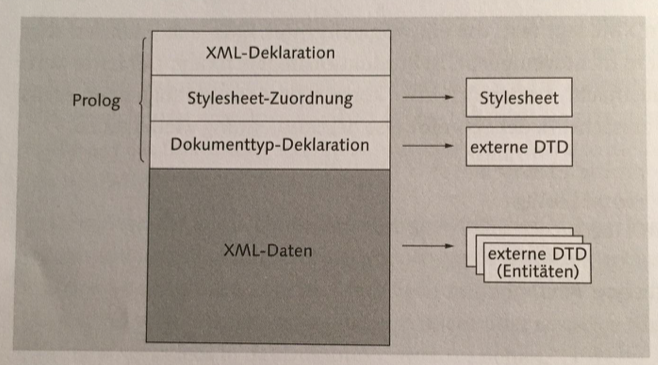
\includegraphics[scale=.5]{./images/Aufbauschema_eines_XML-Dockuments}
\captionof{figure}{Aufbauschema eines XML-Dockuments}

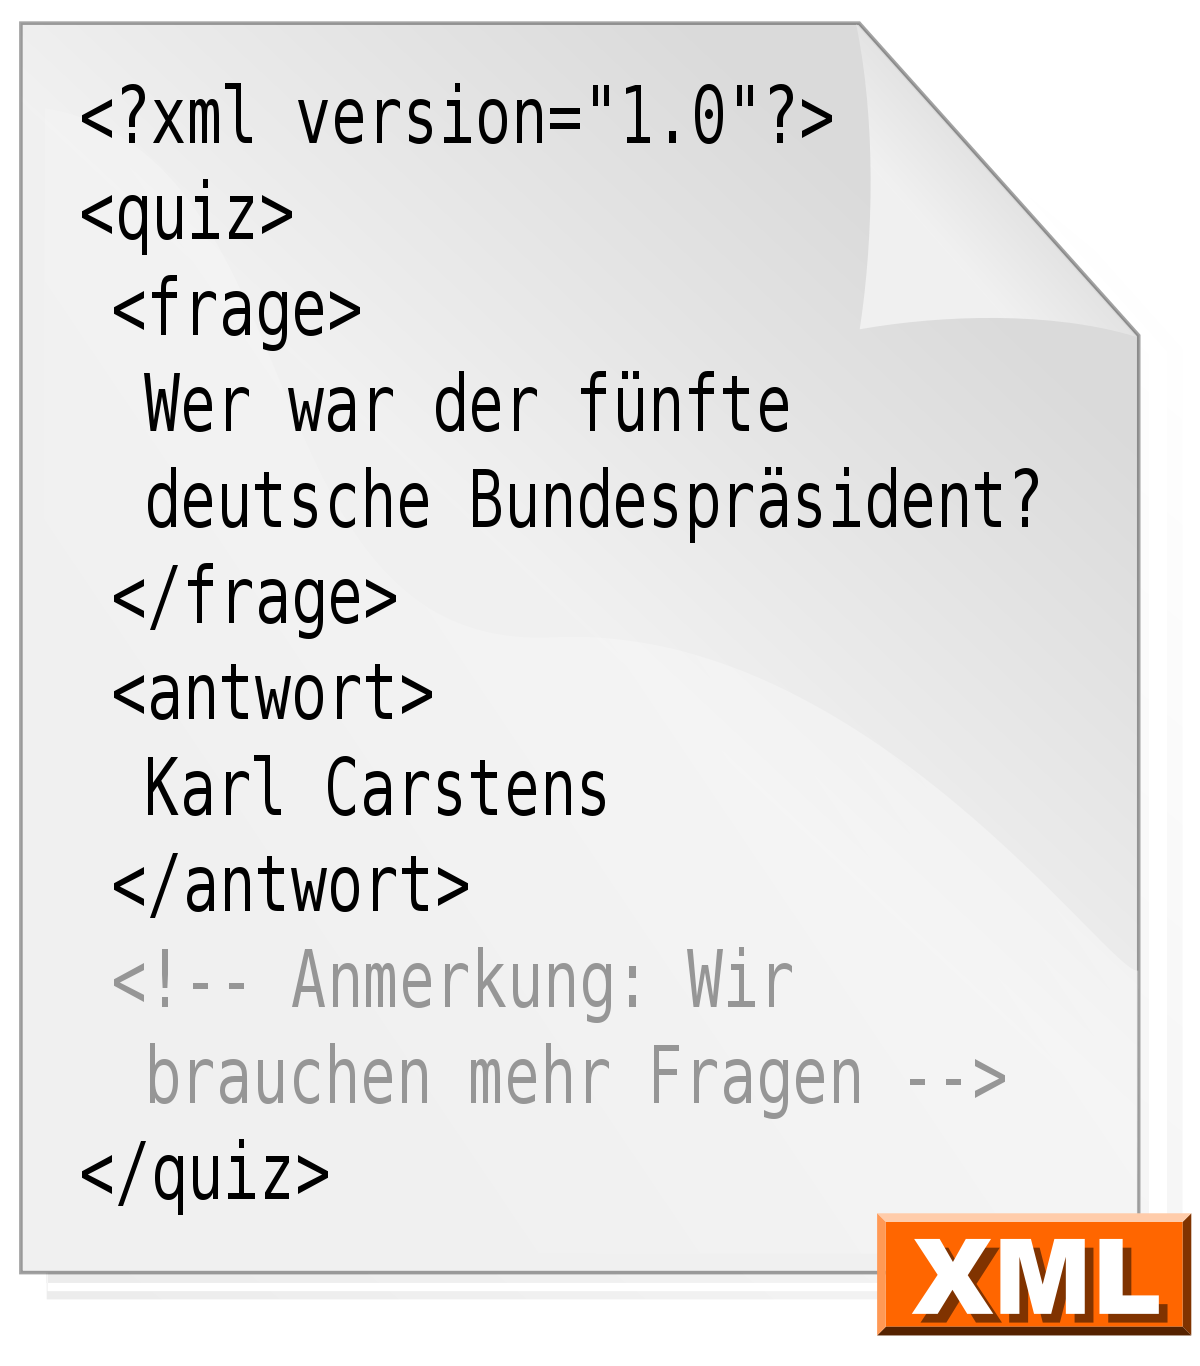
\includegraphics[scale=.3]{./images/Xml_datei_Beispiel}
\captionof{figure}{Beispiel einer XML-Datei}
\end{center}
\subsubsection{JSON}

JSON steht für JavaScript Object Notation und bezeichnet die kompakte Schreibweise von Objekt- und Arraystrukturen.\cite{philipp524} Es handelt sich um ein textuelles Daten Format, das von der Objekt Notation der JavaScript-sprache abgeleitet ist. es wird sehr gerne als Datentransportsprache zwischen Client und Server für Ajax-anfragen verwendet. Für einen schnellen Austausch wird es oft gegenüber XML bevorzugt. Werfen wir zuerst einen Blick auf die Geschichte von JSON. 

\textit{\textbf{Historik}}

Kurz nach Beginn des großen AJAX-Hypes im Jahr 2005 etablierte sich aus praktischen Gründen neben Klartext und XML quasi eine weiteres Übertragungsformat für die Kommunikation via AJAX: JSON, die JavaScript Objekt Notation.\cite{philipp658}
Der JSON wurde von Douglas Crockford zwischen 2002 und 2005 gebaut. Der erste JSON-Standard ist ECMA-404, der im Oktober 20032 veröffentlicht wurde. Derzeit wird er von zwei konkurrierenden Standards beschrieben: IETF RFC 82593 und ECMA-4044. Die neueste Version der Formatspezifikation stammt vom Dezember 2017. \cite{wikip01}

\textit{\textbf{Anwendung}}

Um ein vollständiges und konformes JSON zu erstellen, ist es notwendig, die richtige Syntax zu befolgen und das Dokument mit der Erweiterung .json zu speichern. Ein Json-Objekt beginnt und endet mit geschweiften Klammern {} und besteht im Wesentlichen aus zwei Teilen: Schlüssel und Werte. 

Die Schlüssel sind Zeichenketten, sie enthalten eine Folge von Zeichen, die von Anführungszeichen umgeben sind. Wert ist ein gültiger JSON-Datentyp. Es kann in Form eines Arrays, Objekts, einer Zeichenkette, eines booleschen Wertes, einer Zahl oder null vorliegen. Es kann zwei oder mehr Schlüssel/Wertpaare enthalten, die durch ein Komma getrennt sind. Auf jeden Schlüssel folgt ein Doppelpunkt, um ihn vom Wert zu unterscheiden. Mit diesem Bild ist es möglich, eine Darstellung eines Json zu beobachten. 

\begin{center}
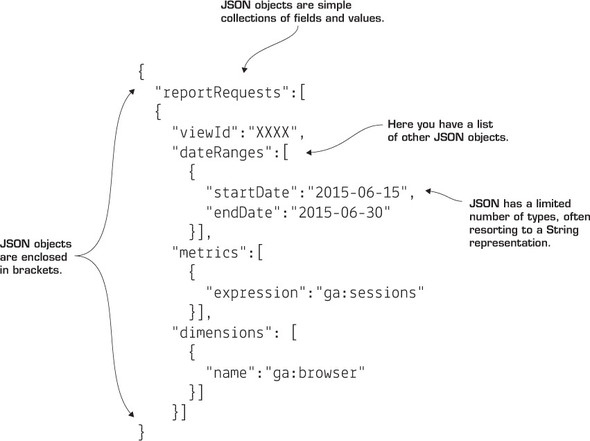
\includegraphics[scale=1]{images/Darstellung_eines_JSON-Objekts}
\captionof{figure}{Darstellung eines JSON-Objekts}
\end{center}

\subsubsection{BSON}

BSON ist eine Weiterentwicklung des Datenaustauschformates JSON der Firma 10gen und ist unter anderem ein fester Bestandteil von MongoDB. Die Libraries sind für viele Programmiersprachen bereits vorhanden. Da die BSON-Spezifikation öffentlich ist, kann BSON auch für andere Projekte genutzt werden.\cite{thKloeln}

BSON ist so konzipiert, dass es im Raum effektiv ist, aber in einigen Fällen ist es nicht viel effektiver als JSON. In einigen Fällen benötigt BSON sogar mehr Platz als JSON. Der Grund dafür ist ein weiteres Designziel von BSON: die Kreuzbarkeit. BSON fügt den Dokumenten zusätzliche Informationen hinzu, wie z. B. die Länge von Strings und Unterobjekten. Dadurch wird die Traversierung schneller.\cite{bson} BSON ist außerdem so konzipiert, dass es sich schnell kodieren und dekodieren lässt. Ganzzahlen werden z. B. als 32- (oder 64-) Bit-Ganzzahlen gespeichert, so dass sie nicht in und aus dem Text geparst werden müssen. Dies verbraucht mehr Speicherplatz als JSON für kleine ganze Zahlen, aber es ist viel schneller zu parsen. Neben der Kompaktheit fügt BSON zusätzliche Datentypen hinzu, die in JSON nicht verfügbar sind, darunter die Datentypen BinData und Date.“
\subsection{Programmierparadigmen für Webanwendungen}
\subsubsection{SOAP}
SOAP steht für Simple Object Access Protocoll und wurde von DevelopMentor, IBM, Lotus Development Corp, Microsoft, Userland Software entwickelt. Der Hauptautor ist Don Box von DevelopMentor, einer der Autoren des XML-Manifests. SOAP ist ein Standard, der vom W3C-Konsortium unterstützt wird. In der Welt der Web-Service-Technologie steht SOAP für ein standardisiertes Paketprotokoll zum Nachrichtenaustausch zwischen verteilten Systemen. Diese Spezifikation definiert eine einfache xml-basierte Umgebung (envelope) zum Austausch von Informationen und einen Satz von Regeln zur Übersetzung von Anwendungen und plattformspezifischen Datentypen in XML-Darstellungen. SOAP ist so konzipiert, dass es eine Vielzahl von Anwendungsfällen unterstützt.\cite{saop1}

\textit{\textbf{Historik}}

Einer der Hauptakteure bei der Emanzipation von Web-Services-Technologien auf der Java-Plattform ist IBM. IBM hat außerdem eine der allerersten Implementierungen der SOAP-Spezifikation für Java auf den Markt gebracht, die in der Java-Entwicklergemeinde auf großes Interesse gestoßen ist. Seitdem konzentriert sich IBM auf die Fähigkeiten dieser Gemeinschaft, um den Erfolg und die Nachhaltigkeit des Frameworks sicherzustellen. Daher beschloss IBM in der zweiten Hälfte des Jahres 2000, SOAP der Open-Source-Welt zu schenken, insbesondere der Apache Fundation.

Das Apache SOAP-Framework von IBM, das in Apache umbenannt wurde, hat eine Reihe von Weiterentwicklungen und Verbesserungen erfahren und war ein großer Erfolg. Infolgedessen hat Sun Apache SOAP schnell als Apache SOAP Framework in seine J2EE-Applikationsserver integriert. Apache SOAP Version 2.2 wurde im Mai 2001 veröffentlicht und danach gab es keine weitere Entwicklung dieses Frameworks. Nachdem das SOAP Framework das Ende seiner Lebensdauer erreicht zu haben scheint, werden sich im kommenden Jahr alle Anstrengungen auf den Nachfolger von Apache SOAP konzentrieren.

\textit{\textbf{Anwendung}}

Die schon im Namen explizit betonte Einfachheit des Protokolls ist dabei ausdrückliches Designziel. Es geht darum, einen unkomplizierten Rahmen für die Nachrichten Übermittlung zwischen Anwendungen bereitzustellen, ohne zu enge Festlegungen über die Art des Nachrichtentransports oder die Anwendungen selbst zu treffen, die das Protokoll nutzen wollen. Dazu wurde eine kleines XML-Vokabular entwickelt, das hauptsächlich angibt, wie die Nachrichten verpackt werden. Ein SOAP-Nachricht ist zunächst ein ganz normales XML-Dokument, das mit den üblichen XML-Prozessoren verarbeitet werden kann. Der Spezifikationsentwurf schreibt als äußeren Rahmen eine <envelope>-Element vor, also einen Umschlag, in den alles andere hineingepackt wird. Optional ist ein SOAP-Header, vorgeschrieben dagegen ein SOAP-Body, der den eigentlichen Inhalt der Nachricht enthält.\cite{helmut529_30}

\begin{center}
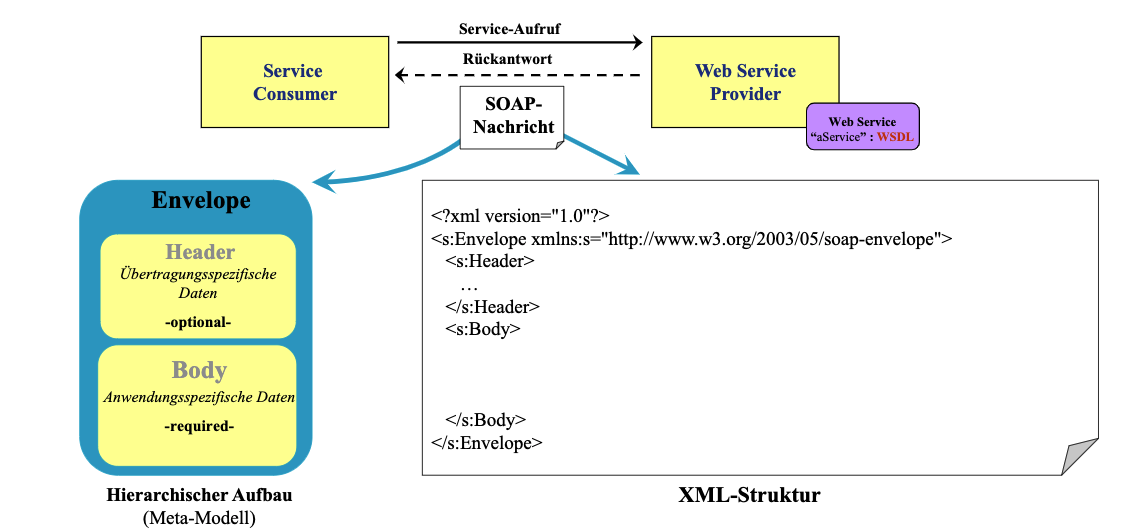
\includegraphics[scale=.4]{images/Struktur_ein_SOAP}
\captionof{figure}{Struktur ein SOAP}
\end{center}

\subsubsection{REST API}
Damit wir die RestFull Api verstehen, fangen wir erst wieder mit den Definitionen ein.
Ein REST stellt einen alternativen Ansatz für die Realisierung von Web Services dar.“ Eine Rest API ist eine Schnittstelle, über die Sie die Kommunikation zwischen Ihrem Computer und einem Server herstellen können, damit dieser Ihnen Daten zur Verfügung stellt. Rest-API ist die an der häufigsten verwendeten Art von API im Webbereich. REST steht für Representational State Transfert.\cite{alda}

\textit{\textbf{Historik}}

Vor den 2000er Jahren gab es keine Standards dafür, wie man eine API entwirft oder gar verwendet. Die Integration von APIs erforderte die Verwendung von Protokollen, wie z. B. SOAP, die notorisch komplex in der Erstellung, Verwaltung und Fehlersuche sind. Das alles änderte sich in den 2000er Jahren, als das wahre Potenzial von Web-APIs erkannt wurde. Eine Gruppe von Experten, angeführt von Roy Fielding, erfand REST und veränderte die API-Landschaft für immer.
Das Ziel war es, einen einfachen Standard zu schaffen, der es zwei Servern ermöglicht, miteinander zu kommunizieren und Daten auszutauschen, egal wo auf der Welt sie sich befinden. Sie schufen eine Reihe von Prinzipien, Eigenschaften und Einschränkungen, die REST genannt werden, sowie eine ressourcen-orientierte Architektur: einheitliche Schnittstelle, Client/Server-Architektur, keines Zustands, Implementierung der Ressourcen-darstellung, Verwendung von HTTP und HTTP-Methoden.

\textit{\textbf{Anwendung}}

Eine API wird oft mit dem Server oder der Datenbank verwechselt, aber in Wirklichkeit handelt es sich um den Code, der den Server anweist, bestimmte Aktionen entsprechend der gestellten Anfrage auszuführen. Es handelt sich also einfach um ein Interface (Application Programming Interface).
Der Zugriff auf den Rest der API erfolgt über HTTP-Methoden (GET, POST DELETE, PUT). Dadurch ist es möglich, einen Server mit einer vom Ersteller der API bereitgestellten URL durch eine einfache HTTP-Anfrage zu interagieren. Eine HTTP-Anfrage an einen Server provoziert jedoch eine Antwort, je nach Erfolg (Code: 200) oder Misserfolg der Operation (403, 404, 500, 504 ...). Es ist möglich, die Daten Allgemeinen im JSON-Format zu erhalten.

\begin{center}
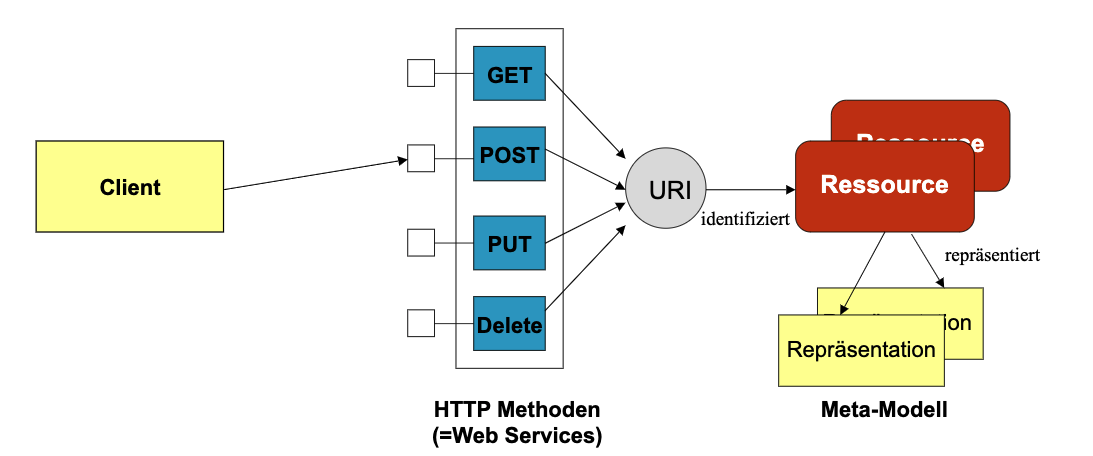
\includegraphics[scale=.3]{images/Aufbau_eine REST-basierten_Web_Services_Architektur}
\captionof{figure}{Aufbau eine REST-basierten Web Services Architektur}
\end{center}

\subsubsection{GraphQL}

GraphQL ist eine Abfragesprache für APIs und eine Laufzeitumgebung zur Erfüllung dieser Abfragen mit Ihren vorhandenen Daten. GraphQL bietet eine vollständige und verständliche Beschreibung der Daten in Ihrer API, gibt Kunden die Möglichkeit, genau das anzufordern, was sie benötigen, und nicht mehr, erleichtert die Weiterentwicklung von APIs im Laufe der Zeit und ermöglicht leistungsstarke Entwicklerwerkzeuge.\cite{graphQL}

\textit{\textbf{Historik}}

Bis 2012 wird die Verbreitung von Mobiltelefonen weltweit monströse Zahlen erreichen. Es ist eine solche Invasion, dass Unternehmen, die ihre Produkte nicht anpassen, gefährdet sind. An diesem Punkt ist Facebook gefährdet. Facebook geht online. Als Ergebnis haben sie ihre IOS-App wie eine Website gemacht, in Web-Ansicht. Sehr schnell merken sie, dass es (zu diesem Zeitpunkt) ein bisschen scheiße ist. Also entschied man sich, es komplett in nativer Sprache neu zu erstellen, um ein besseres Kundenerlebnis zu schaffen. Sofort wurde ihnen eine weitere Wand vor die Nase gesetzt. Die bestehende Architektur funktioniert nicht. Hauptsächlich, weil die Endpunkte ihrer bestehenden REST-API keine Flexibilität bei den Daten zulassen. Für verschachtelte Daten sind mehrere Roundtrips zu verschiedenen Endpunkten erforderlich, was zu Langsamkeit und Inkonsistenzen führt. Ein Teil der Nutzdaten wird für die meisten Abfragen nicht benötigt, was zu unnötigen Datenübertragungen führt. Und vor allem ist es für Facebook mühsam, so viele HTTP-Aufrufe zu verarbeiten.
In diesem infernalischen Kontext reservieren Lee Byron, Dan Schafer und Nick Schrock im Februar 2012 Büros in einer Ecke von Facebook. Sehr schnell wird ein erster Prototyp von GraphQL, damals SuperGraph genannt, von unseren drei Entwicklern erstellt. Im August 2012 wird GraphQL in der Produktion mit der neuen nativen Facebook-App ausgeliefert. Im Jahr 2015 erscheint die erste öffentliche Version im Internet. GraphQL ist auch heute noch präsent, wenn Sie auf Ihrer Facebook-Pinnwand scrollen.\cite{graphQL2}

\textit{\textbf{Anwendung}}

Mit GraphQL kann man Daten auf einfache, flexible und sehr präzise Weise manipulieren. GraphQL ist keine Programmiersprache und kein Framework, sondern eine Spezifikation zur Implementierung einer API.
GrapQL macht das Leben einfacher, denn damit müssen Sie nur eine Post request Anfrage stellen, die nach genau dem fragt, was man genau braucht, als Antwort gibt es die Ressourcen zurück, die nach dem Aufbau Ihres GraphQL Anfrage. Der kleine Unterschied zu REST ist, dass man bei REST von den Endpunkten definierte Objekte bekommt, bei GraphQL hingegen passt man sich nicht an ein vom Backend bereits vordefiniertes Objekt an, sondern man definiert dynamisch, was man auf der Frontend Seite erhalten möchte. 
Das folgende Bild von der Startseite der offiziellen GrapQL-Website stellt die Funktion von GraphQL übersichtlich und einfach dar.

\begin{center}
\includegraphics[scale=.4]{images/Globaler_ueberblick über_GraphQL}
\captionof{figure}{Globaler Überblick über GraphQL}
\end{center}



\chapter{Kapitel II - NoSQL - Ausgewählte Systeme at a Glance}
\section{ArangoDB}
\begin{tabular}{|c|c|}
\hline 
Allgemein \\ 
\hline 
Name & • \\ 
\hline 
Kategorie & • \\ 
\hline 
Version & • \\ 
\hline 
Historie & • \\ 
\hline 
Hersteller & • \\ 
\hline 
Lizenz & • \\ 
\hline 
Quellenangebaen, Download & • \\ 
\hline 
Besonderheiten \\ 
\hline 
• & • \\ 
\hline 
• & • \\ 
\hline 
• & • \\ 
\hline 
• & • \\ 
\hline 
• & • \\ 
\hline 
• & • \\ 
\hline 
\end{tabular} 

\chapter{Kapitel III - NoSQL - Ausgewählte Systeme Unboxed}
\section{ArangoDB}
ArangoDB ist gehört zu den \ac{NoSQL} Datenbanken. Die Datenbank ist besonders bekannt für ihr Multi-Modell. Multi-Modell bedeutet, dass ein \ac{DBS} mehrere Datenmodelle besitzt. Welche diese sind und wie ArangoDB funktioniert und aufgebaut ist, wird in diesem Kapitel erörtert.
\subsection{Anwendungsumfeld}
In vielen Softwareprojekten steht am Anfang nicht fest welches \ac{DBS} das beste für sie sei. Jede Datenbank bringt seine eigenen Vorteile und Nachteile mit sich. Und genau an dieser Stelle spielt ArangoDB eine wichtige Rolle:
Durch sein ’natives’ Multi-Modell ermöglicht es die Vor- und Nachteile von Datenbankmodellen auszugleichen. Dadurch wird ArangoDB zur ’Multi-Purpose-Datenbank’ mit einem dokumentenbasierten Basismodell\cite{jaxenter01}. Es kann bei einer agilen Vorgehensweise mit stetig wechselnden Anforderungen sehr Vorteilhaft sein, ein ebenso flexibles DBS wie ArangoDB zu verwenden.

 \subsection{Technologische Aspekte}
Der Kern der ArangoDB ist sein vielseitiges Multi-Modell, welches insgesamt aus drei verschiedenen Datenbank-Modellen besteht. Diese sind zu einem Modell vereint und können je nach Anwendungsfall eingesetzt werden. Das Multi-Modell besteht aus folgenden  vereinten Datenbankmodellen:

\paragraph{Das dokumentbasierte Modell} dient als solide Basis für das \ac{DBS}. Im Modell wird \ac{JSON} als Speicherformat verwendet. Durch seine Semi-Struktur und hirarschichen Aufbau ist  ein dokumentenbasiertes Modell für viele Anwendungsfälle geeignet\cite{AWS_doc}.  Außerdem bietet es eine gute Grundlage für die beiden anderen Datenmodelle.

\paragraph{Das graphbasiertes Modell} bietet die Möglichkeit Beziehungen zwischen Objekten im dokumentenbasierten Modell abzubilden. Außerdem hilft das graphbasierte Modell Datenstrukturen leichter zu verstehen und JOINs schneller aufzulösen \cite{AWS_graph}. Des Weiteren können sogennante Super-Nodes identifiziert und anschließen optimiert werden, damit der Zugriff auf diese Objekte performanter ist.

\paragraph{Das Key-Value-Modell} ist dafür optimiert Objekte zu einen gewissen Schlüssel schell abzurufen.  Anstatt lange Querys schreiben zu müssen, hilft das Key-Value-Modell optimiert auf diese Werte zuzugreifen. Optimal partitionierte Datensätze durch den geschaffenen Index sind dabei ein großer Vorteil. \cite{AWS_keyvalue}

Zusammenfassend kann man sagen, dass ArangoDB durch die Kombination der drei Datenbankmodellen ein perfektes Modell für fast jeden Anwendungsfall vorweist. Allerdings hat die Vereinigung der Modelle auch Nachteile. ArangoDB bietet zwar dem Nutzer das passende Modell für seinen Anwendungsfall, hat jedoch keine Chance gegenüber der Performance von Datenbanken, die diese Modelle nativ implementieren \cite{ADB_benchmark}.

\subsubsection{Systemarchitektur}
ArangoDB erfüllt im Clusterbetrieb das "CP" des CAP-Theorems \cite{CAP}. Mit seinem Prinzip des 'Master/Master'-Ansatzes ermöglicht es eine hohe Partitionsmöglichkeit und liefert immer die aktuellsten Daten zurück. Ermöglicht wird dies durch die Bereitstellung der drei verschiedenen Komponenten im Clusterbetrieb \cite{ADB_clusterarch}:
\paragraph{Agenten} 
beinhalten die Konfiguration des Clusters. Agenten wissen wie viele DB-Server im Cluster verfügbar sind, wo sich diese befinden und welche Daten diese enthalten. Außerdem kümmern sie sich im synchronität der verschiedenen Datenbankinstanzen im Cluster. Demnach führen diese Komponenten auch Transaktionen auf dem Datenbankcluster aus. Von dem ArangoDB-Team werden Agenten auch als Herz des Clusters bezeichnet. \cite{ADB_clusterarch}
\paragraph{Koordinatoren} bilden die Schnittstelle zum Cluster. Sie kümmern sich um Abfragen mit \ac{AQL} an die Datenbanken oder implementieren Foxx Microservices in ihrer Architektur. Die Koordinatoren wissen, welcher der optimalste Weg für die Datenabfrage ist und sammeln so die Daten von verschiedenen Datenbankservern. Da Koordinatoren zustandlos sind, können diese sehr schnell zu einem bestehen Cluster hinzugefügt werden um Anfrageengpässe verhindern. \cite{ADB_clusterarch}
\paragraph{DB-Server} 
Diese Komponente im Cluster ist für die tatsächliche Datenspeicherung zuständig. An diese Komponente stellen die Koordinatoren ihre Datenabfragen. Bei Datenänderungen werden zunächst die Daten der Hauptdatenbank geändert, um anschließend synchron die Follow-Datenbanken zu aktualisieren.

\begin{figure}[htbp] 
  	\centering
     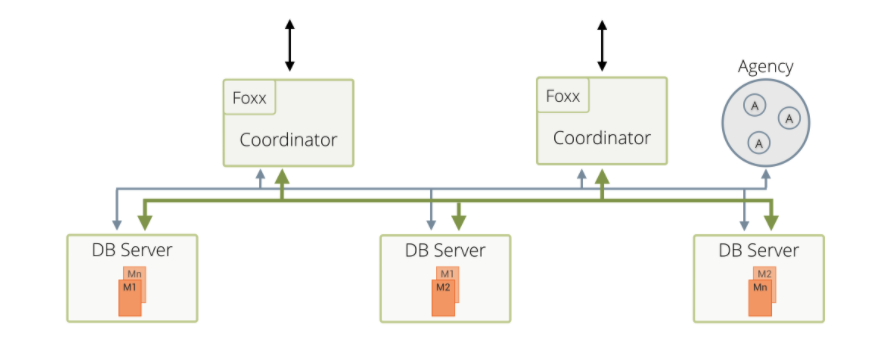
\includegraphics[width=1\textwidth]{./images/cluster-arch.png}
 	\caption{ArangoDB Cluster Architektur \cite{ADB_clusterarch}}
  \label{fig:ClusterArch}
\end{figure}


\subsubsection{Programmierschnittstellen}
ArangoDB bietet eine Vielzahl an Zugriffsmöglichkeiten.

Eine Option sind Treiber für verschiedene Programmiersprachen wie Java, NodeJS, PHP und viele andere. Des Weiteren gibt es Treiber, die von der ArangoDB Community zur Verfügung gestellt werden. \cite{ADB_driver} Diese Führen dann mit \ac{AQL} Datenabfragen auf das Cluster. 

Eine weitere Möglichkeit ist das mitgelieferte \ac{CLI}-Tool 'arangosh'. Ein einfaches Tool, welches bei Installation mitgeliefert wird, um schnelle Testabfragen an das Datenbanksystem zu stellen, jedoch ungeeignet für Produktivsysteme. \cite{ADB_arangosh}

Als letzte Zugriffsmöglichkeit bietet ArangoDB ein \ac{API}. Damit können zum Beispiel Collections, Datenbanken und Kanten über \ac{HTTP} abgefragt werden. \cite{ADB_api} Diese \ac{API} ist erweiterbar um sogennante Foxx-Microservices. Die Microservices werden in das Datenbanksystem mittels Javascript deployed. Foxx-Microservices dienen dem Nutzer der Datenbank, komplexere Berechnungen oder Abfragen datenbanknahe und optimiert auszuführen. \cite{ADB_foxx}

\subsection{Datenbankentwicklung}
\subsubsection{Systeminstallation}
Um die ArangoDB auf einen Linux Server zu installieren folgt man den Anweisungen auf der Webseite von ArangoDB.

Als ersten Schritt muss ein Repository-Schlüssel dem Paket-Manager \texttt{apt} hinzugefügt werden.
\begin{lstlisting}[language=bash]
curl -OL https://download.arangodb.com/arangodb37/DEBIAN/Release.key
sudo apt-key add - < Release.key
\end{lstlisting}
Anschließend kann über den Paketmanager die Installation folgen:
\begin{lstlisting}[language=bash]
echo 
	'deb https://download.arangodb.com/arangodb37/DEBIAN/ /' | 
	sudo tee /etc/apt/sources.list.d/arangodb.list
sudo apt-get install apt-transport-https
sudo apt-get update
sudo apt-get install arangodb3=3.7.3-1
\end{lstlisting}
Nachdem die Installation abgeschlossen wurde, kann der automatisch gestartete ArangoDB-Services wieder gestoppt werden. Diese Schritte werden nacheinander auf allen vier Nodes im Cluster ausgeführt. \cite{ADB_install}

Um nun einen ArangoDB-Cluster zu starten, haben wir den ArangoDB Starter verwendet. Der Starter ist ein \ac{CLI}-Tool, welches über Parameter die Optionen eines Datenbankservers konfiguriert. 
Für unseren Cluster haben wir für den Hauptserver (Node-4) folgende Konfiguration gewählt:
\begin{lstlisting}[language=bash]
sudo arangodb \
--starter.data-dir=/data/team38 \
--server.storage-engine=rocksdb
\end{lstlisting}
Alle weiteren Nodes wurden mit diesem Befehl mit dem Datenbankserver von Node-4 verbunden:
\begin{lstlisting}[language=bash]
sudo arangodb \
--starter.join c017-node4 \
--starter.data-dir=/data/team38 \
--server.storage-engine=rocksdb
\end{lstlisting}
\citep{ADB_starter}


\subsubsection{Datenmodellierung und Beispielschema}
Um den Use Case für den Graphen so verständlich wie möglich zu gestalten, haben wir uns ein einfaches Schema entschieden. Es besteht aus genau zwei Entitäten. Eine Collection, welche Autodaten enthält und eine weitere Collection, die die Kanten für unseren Graphen enthält. Diese Kanten zeigen von einer Auto-Entität auf eine andere Auto-Entität.
\begin{figure}[htbp] 
  	\centering
     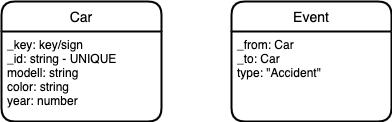
\includegraphics[width=.7\textwidth]{./images/Schema.png}
 	\caption{Implementiertes Beispielschema}
  \label{fig:DataSchema}
\end{figure}
\subsubsection{Import der Beispieldaten}
Über das Webinterface der Datenbank lassen sich für jede Collection über ein \ac{JSON}-Import Daten importieren.
Ausschnitt von Car Beispieldaten:
\lstinputlisting[linerange={1-9}, caption=Beispieldaten Auto, label=Beispieldaten Auto]{./json/cars.json}
Ausschnitt von Event Bespieldaten:
\lstinputlisting[linerange={1-9}, caption=Beispieldaten Event, label=Beispieldaten Event]{./json/events.json}
\subsubsection{AdHoc-Anfragen}
\begin{figure}[htbp] 
  	\centering
     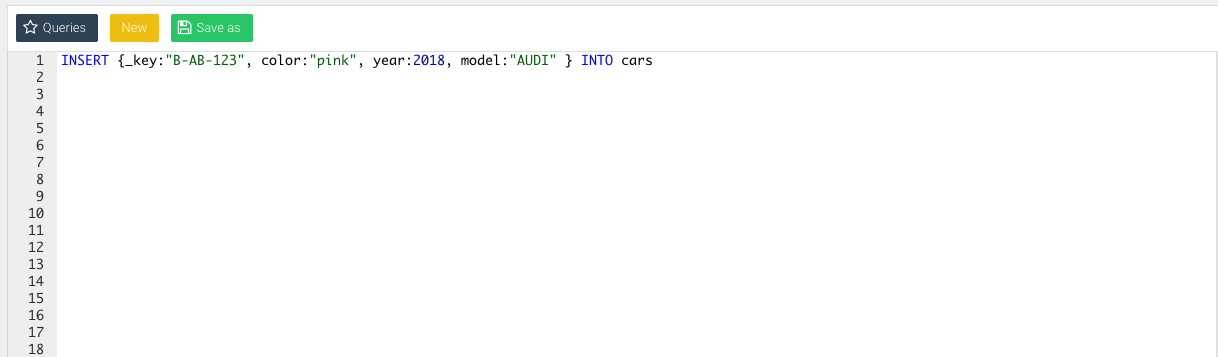
\includegraphics[width=1\textwidth]{./images/create.png}
 	\caption{CREATE von Dokument im Schema}
  \label{fig:DataSchema}
\end{figure}
\begin{figure}[htbp] 
  	\centering
     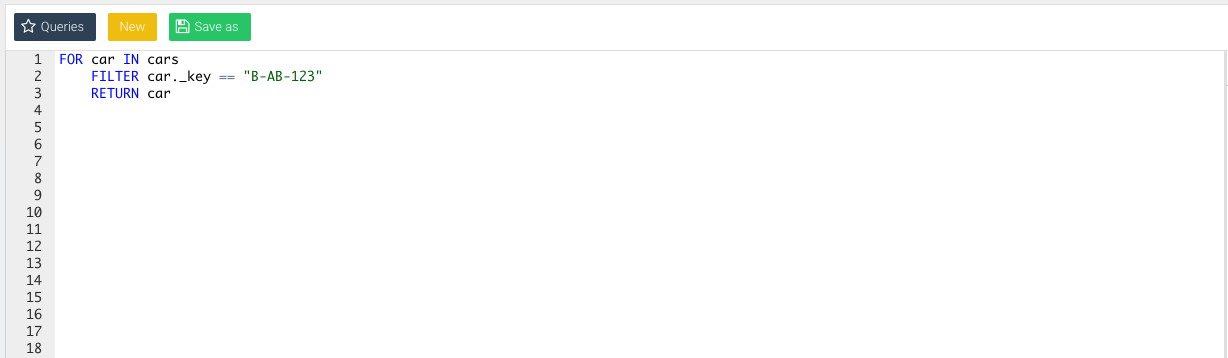
\includegraphics[width=1\textwidth]{./images/select.png}
 	\caption{SELECT vom erstellten Dokument}
  \label{fig:DataSchema}
\end{figure}
\begin{figure}[htbp] 
  	\centering
     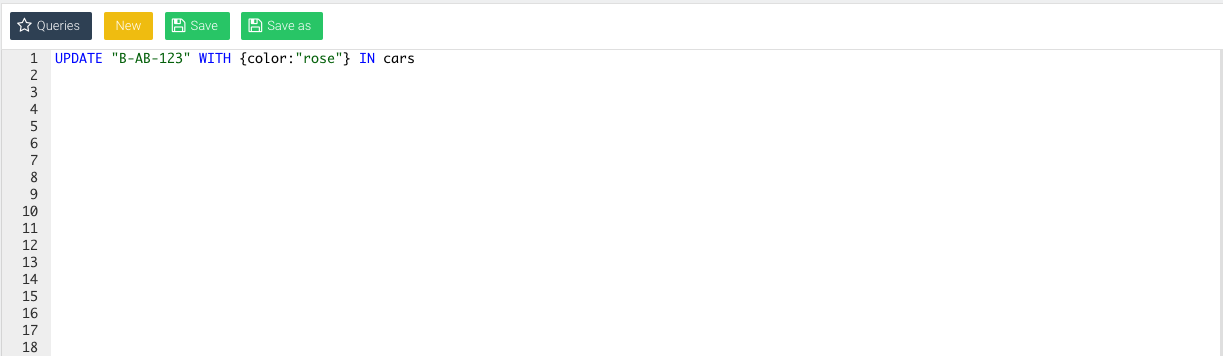
\includegraphics[width=1\textwidth]{./images/update.png}
 	\caption{UPDATE vom erstellten Dokument}
  \label{fig:DataSchema}
\end{figure}
\begin{figure}[htbp] 
  	\centering
     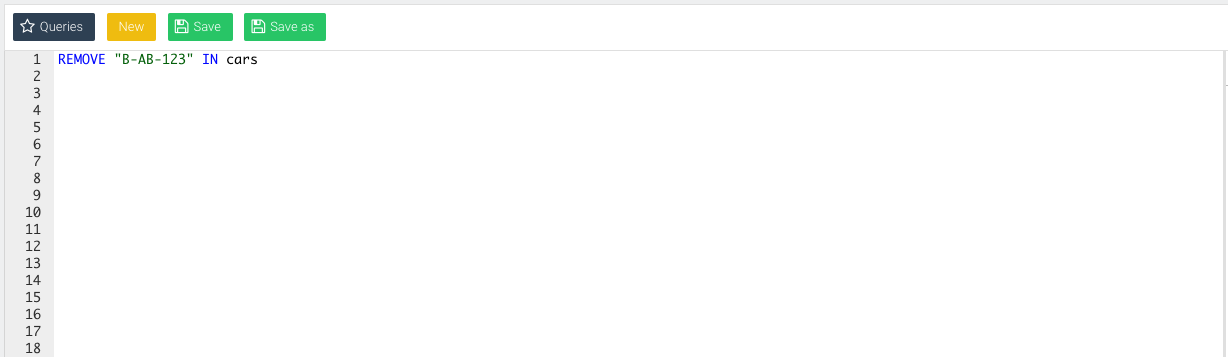
\includegraphics[width=1\textwidth]{./images/delete.png}
 	\caption{DELETE vom erstellten Dokument}
  \label{fig:DataSchema}
\end{figure}
\chapter{Kapitel IV - NoSQL – Ausgewählte Systeme in Action}
\section{ArangoDB}

\subsection{Implementierung von Anwendungsszenarien}
\subsubsection{FunktionalitätdesAnwendungsszenarios}
\subsubsection{Mögliche Experimente mit dem Clusterbetriebs}
\subsubsection{Mögliche Experimente mit der Transaktionsverarbeitung}
\subsubsection{Mögliche Experimente mit der Leistungsbewertung}

\subsection{Implementierungskonzept}

\subsection{Anwendung und Test}

\subsection{Fazit}
\chapter{Kapitel V - Fazit}
\setcounter{section}{7}
\section{ArangoDB}

\newpage

% loads the fancy pagestyle for register part
% set the pagestyle to fancy
\pagestyle{fancy}

\fancyhf{}% clear all fields
  % define the header
  \fancyhead[L]{\leftmark}% left header
  \fancyhead[R]{\HEADER}% right header
  \renewcommand{\headrulewidth}{0.4pt}% top line

  % define the footer
  \fancyfoot[L]{\AUTHOR}% left footer
  \fancyfoot[R]{\pagemark}% right footer
  \renewcommand{\footrulewidth}{0.6pt}% bottom line

  % redefine the chaptermark to have '1. Chaptername' and not 'CHAPTER 1.
  % CHAPTERNAME'
  \renewcommand{\chaptermark}[1]{\markboth{\thechapter.\ #1}{}}

% override the plain style
\fancypagestyle{plain}{%
\fancyhf{}% clear all fields
  % define the header
  \renewcommand{\headrulewidth}{0.0pt}% top line

  % define the footer
  \fancyfoot[L]{\AUTHOR}% left footer
  \fancyfoot[R]{\pagemark}% right footer
  \renewcommand{\footrulewidth}{0.6pt}% bottom line
}


% #####
% # load the appendix from the files
% #####
\appendix
\chapter{Name: ArangoDB}
\section{Versuchsergebnisse}
\begin{figure}[htbp] 
  	\centering
     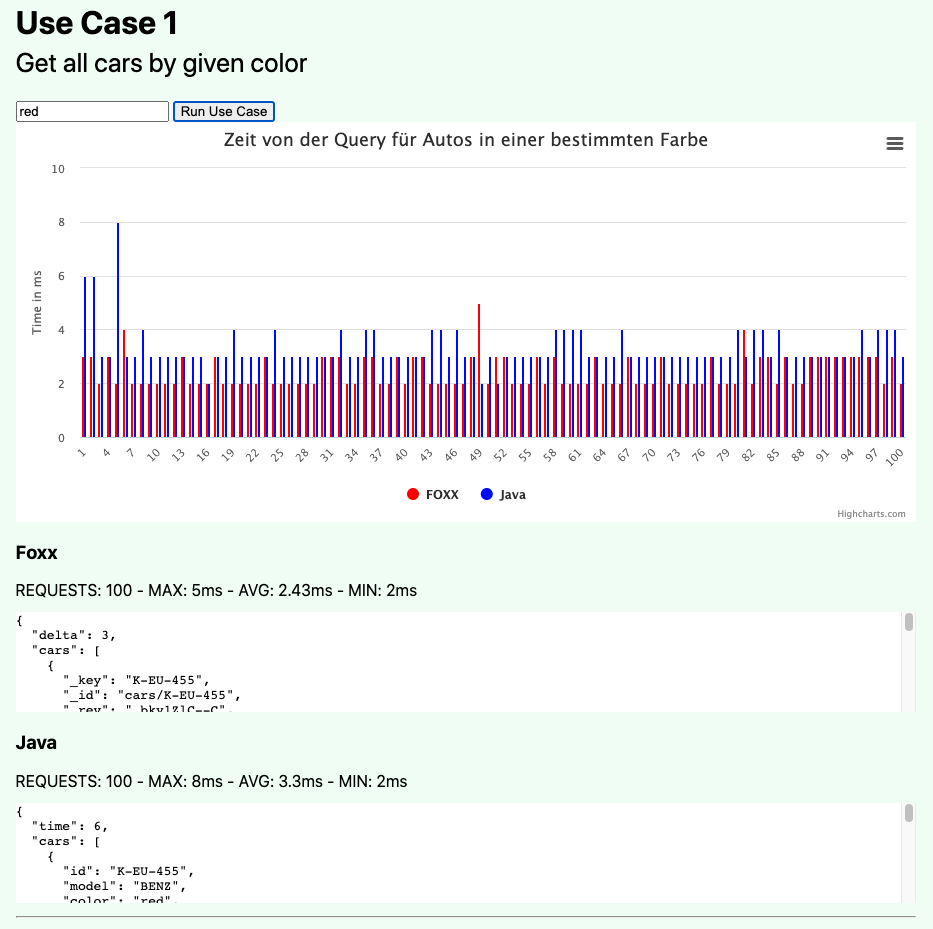
\includegraphics[width=1\textwidth]{./images/8.UseCase1.png}
 	\caption{Anwendungsszenario 1 Ergebnisse}
  \label{fig:DataSchema}
\end{figure}

\begin{figure}[htbp] 
  	\centering
     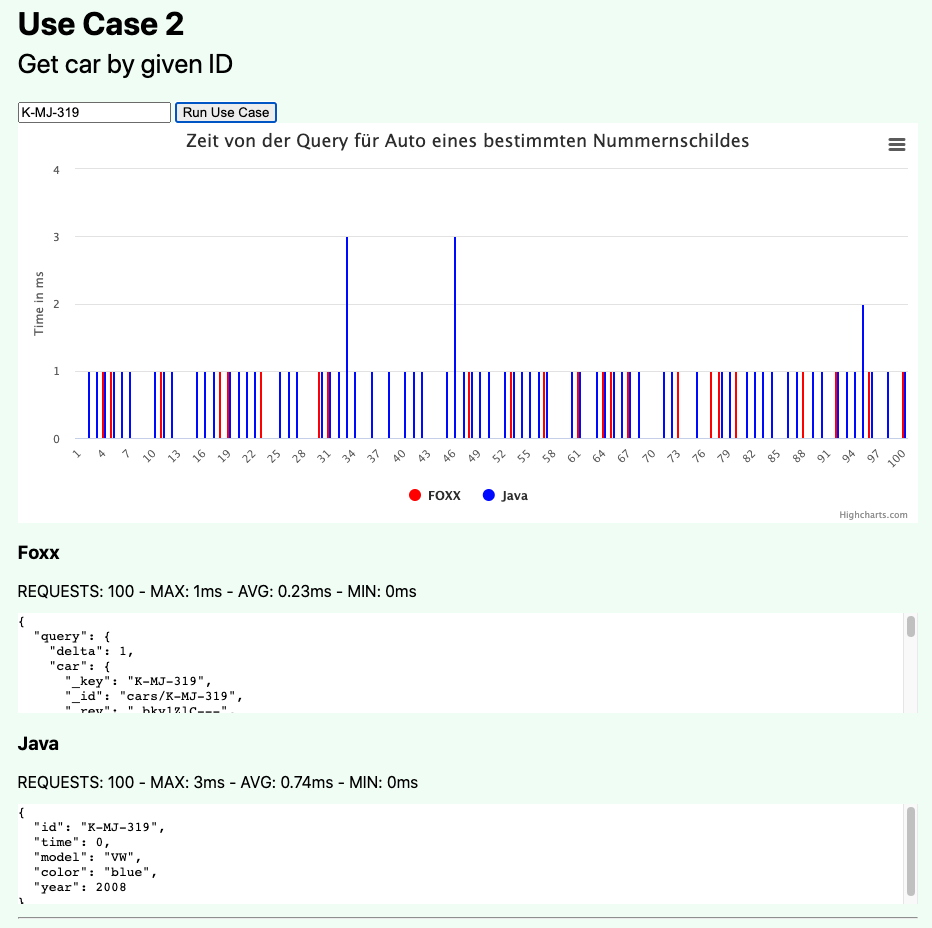
\includegraphics[width=1\textwidth]{./images/8.UseCase2.png}
 	\caption{Anwendungsszenario 1 Ergebnisse}
  \label{fig:DataSchema}
\end{figure}

\begin{figure}[htbp] 
  	\centering
     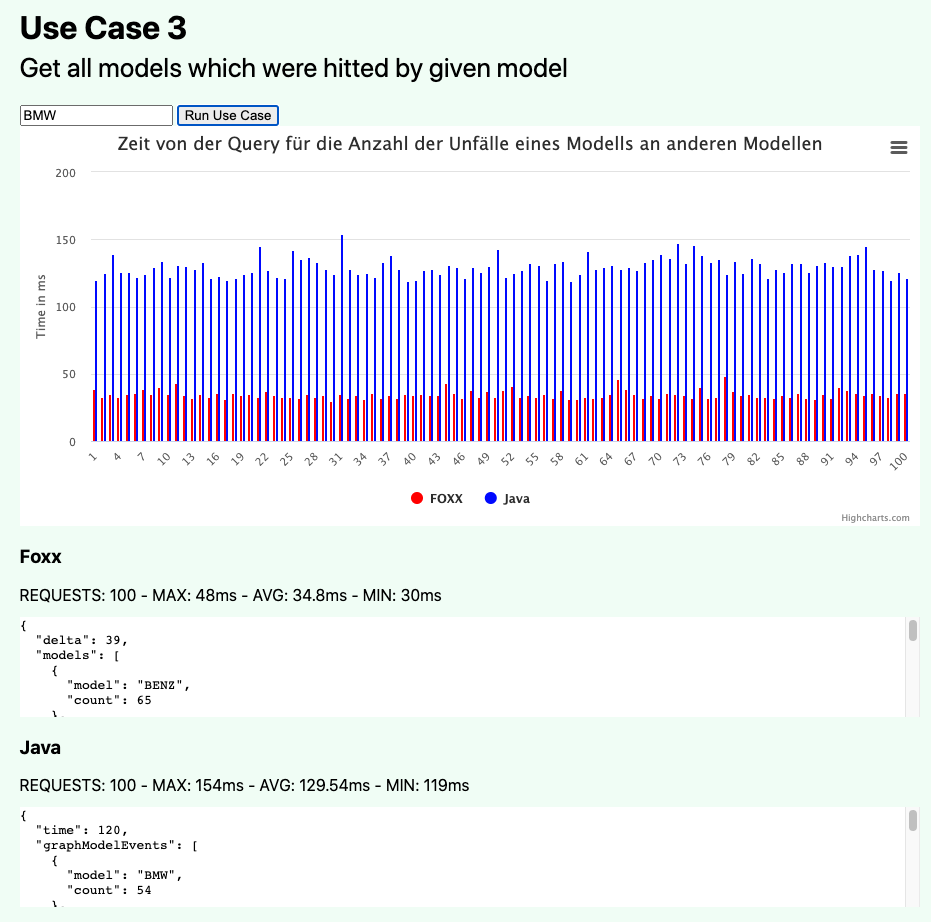
\includegraphics[width=1\textwidth]{./images/8.UseCase3.png}
 	\caption{Anwendungsszenario 1 Ergebnisse}
  \label{fig:DataSchema}
\end{figure}



% #####
% # list of table, list of figures, and list of listings in ToC
% #####
\newpage
\addcontentsline{toc}{chapter}{Abbildungsverzeichnis}
\listoffigures
\newpage
\addcontentsline{toc}{chapter}{Tabellenverzeichnis}
\listoftables
\newpage
\addcontentsline{toc}{chapter}{Listings}
\lstlistoflistings

% #####
% # List of Abbreviations
% #####
\phantomsection 
\addcontentsline{toc}{chapter}{Abkürzungsverzeichnis}
\renewcommand\refname{Abkürzungsverzeichnis} 
\chapter*{Abkürzungsverzeichnis}
\begin{acronym}[RDBMS] % längste Abkürzung steht in eckigen Klammern
    \setlength{\itemsep}{-\parsep} % geringerer Zeilenabstand
    \acro{API}{Application Programming Interface}
    \acro{BASE}{Basically Available, Soft State, Eventual Consistency}
    \acro{BG}{Barahmand Ghandeharizadeh}
    \acro{CAP}{Consistency Availibiltiy Partition Tolerance}
    \acro{CLI}{Command-Line Interface}
    \acro{CPU}{Central Processing Unit}
    \acro{CRUD}{Create, Read, Update, Delete}
    \acro{DBA}{Datenbankadministrator}
    \acro{DBS}{Datenbanksystem}
    \acrodefplural{DBS}[DBS]{Datenbanksysteme}
    \acrodefplural{HDD}[HDDs]{Hard Disk Drive}
    \acrodefplural{SSD}[SSDs]{Solid State Drive}
    \acro{DNS}{Domain Name System}
    \acro{DTD}{Document Type Definition}
    \acro{GUI}{Graphical User Interface}
    \acro{HDD}{Hard Disk Drive}
    \acro{IP}{Internet Protocol}
    \acro{JDBC}{Java Database Connectivity}
    \acro{JSON}{JavaScript Object Notation}
    \acro{NoSQL}{Not only SQL}
    \acro{OLTP}{Online Transaction Processing}
    \acro{RDBMS}{Relational Database Management System}
    \acro{RFC}{Request For Comments}
    \acro{SLA}{Service Level Agreement}
    \acro{SPEC}{Standard Performance Evaluation Corporation}
    \acro{SQL}{Structured Query Language}
    \acro{SSD}{Solid State Drive}
    \acro{TPC}{Transaction Processing Performance Council}
    \acro{UML}{Unified Markup Language}
    \acro{XML}{Extensible Markup Language}
    \acro{YCSB}{Yahoo! Cloud Serving Benchmark}
\end{acronym}

\newpage

% #####
% # load the bibliography
% #####
\bibliography{bibliography}

% #####
% # load the sworn declaration
% #####
\chapter*{Eidesstattliche Erklärung}\markboth{Eidesstattliche Erklärung}{}
  \addcontentsline{toc}{chapter}{Eidesstattliche Erklärung}
Ich versichere an Eides Statt durch meine eigenhändige Unterschrift, dass
ich die vorliegende Arbeit selbstständig und ohne fremde Hilfe angefertigt
habe. Alle Stellen, die wörtlich oder dem Sinn nach auf Publikationen oder
Vorträgen anderer Autoren beruhen, sind als solche kenntlich gemacht.
Ich versichere außerdem, dass ich keine andere als die angegebene
Literatur verwendet habe. Diese Versicherung bezieht sich auch auf alle in
der Arbeit enthaltenen Zeichnungen, Skizzen, bildlichen Darstellungen und
dergleichen.
\\
\\
Die Arbeit wurde bisher keiner anderen Prüfungsbehörde vorgelegt und
auch noch nicht veröffentlicht.
\vspace{3cm}

\centering
\begin{tabular}{p{10mm}>{\centering\arraybackslash}p{50mm}p{10mm}
>{\centering\arraybackslash}p{50mm}p{10mm}}
&\textit{\large \TOWN,}&&& \\
&\textit{\large den \today}&&\hrulefill& \\
&\small Ort, Datum&&\small \AUTHOR&
\end{tabular}
% end of the document
\end{document}
